%
% File acl2014.tex
%
% Contact: koller@ling.uni-potsdam.de, yusuke@nii.ac.jp
%%
%% Based on the style files for ACL-2013, which were, in turn,
%% Based on the style files for ACL-2012, which were, in turn,
%% based on the style files for ACL-2011, which were, in turn, 
%% based on the style files for ACL-2010, which were, in turn, 
%% based on the style files for ACL-IJCNLP-2009, which were, in turn,
%% based on the style files for EACL-2009 and IJCNLP-2008...

%% Based on the style files for EACL 2006 by 
%%e.agirre@ehu.es or Sergi.Balari@uab.es
%% and that of ACL 08 by Joakim Nivre and Noah Smith

\documentclass[11pt]{article}
\usepackage{acl2014}
\usepackage{times}
\usepackage{url}
\usepackage{latexsym}
\usepackage{graphicx}

%\setlength\titlebox{5cm}

% You can expand the titlebox if you need extra space
% to show all the authors. Please do not make the titlebox
% smaller than 5cm (the original size); we will check this
% in the camera-ready version and ask you to change it back.


\title{Recursive Neural Network Part-of-Speech Tagger}

\author{Hao Liu \\
  NYU \\
  {\tt email@domain} \\\And
  Jiali Huang \\
  NYU \\
  {\tt email@domain} \\\And
  Robert Dionne \\
  NYU \\
  {\tt robertsdionne@nyu.edu} \\}

\date{}

\begin{document}
\maketitle
\begin{abstract}
  TODO: Write the abstract
\end{abstract}

\section{Introduction}

For our final project, we implemented a recursive neural network part-of-speech tagger based on similar prior work by Socher, Manning and Ng (2010) for building sentence parse trees and work by Collobert and Weston (2011) for their distributed word representations. We wanted to explore natural language processing using neural networks, so we chose a small problem (part-of-speech tagging) which we already had experience with during the third homework assignment and applied these modern techniques in neural network research to the problem.

Recursive neural networks are neural network models that allow for cyclic connections between neurons. 

\section{Our Models}

TODO: Write about our models.

\subsection{Basic}

TODO: Describe models.

\subsection{Compositional Vector Grammar}

TODO: Describe CVG.

\subsection{Future}

TODO: Describe future models.

\section{Experiments}

TODO: Describe experiments.

\subsection{Backpropagation Through Time}

TODO: Describe back propagation through time.

\subsection{Training Tricks}

TODO: Describe training tricks.

\subsubsection{Weight Initialization}

TODO: Describe weight initialization.

\subsubsection{AdaGrad}

TODO: Describe AdaGrad.

\subsection{Analysis}

TODO: Describe analysis.

\subsubsection{Training Progress Diagram}

TODO: Describe training progress diagrams.

\subsubsection{Comparison to Other Models}

TODO: Compare to baseline.

TODO: Compare to HMM.

\subsubsection{Error Analysis}

\paragraph{Confusion matrices} 
We plot the confusion matrix(Figure \ref{Conf_fig}) for the basic RNN model and find that:
\begin{enumerate}
\item The \textbf{most serious confusion is between NNP and NN}. This makes sense, because the fact that the embemdings we are using make no difference between captitaled word and noncapitaled word;
\item  Another strange confusion is from quotes, which was also met in common HMM models. These may come from the overwhelming sequential information;
\item Other confusions look normal, and also occur in HMM models, like JJ and NN.
\end{enumerate}
\begin{figure}
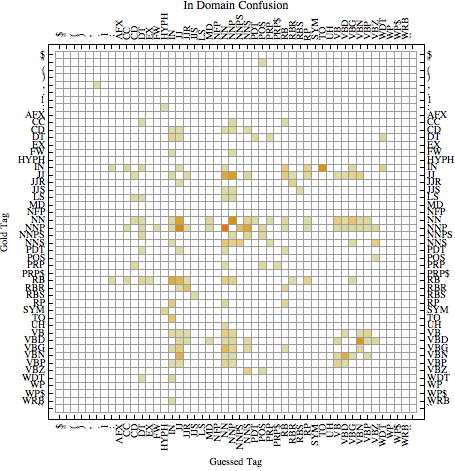
\includegraphics[scale=0.5]{indomain_conf.png} 
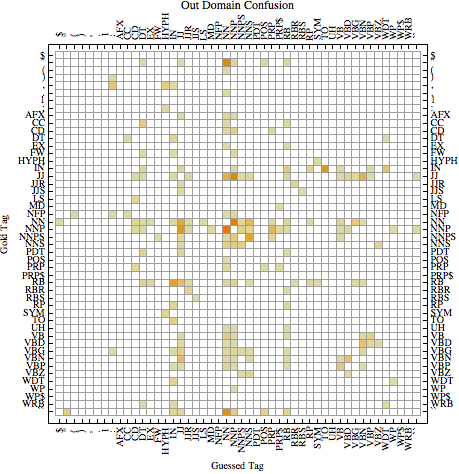
\includegraphics[scale=0.5]{outdomain_conf.png} 
\caption{Confusion matrices for basic RNN}\label{Conf_fig}
\end{figure}



\paragraph{Position of wrong tags } 
We plot the histogram(Figure \ref{Pos_fig}) of related position(absolute positon in sentence divided by sentence length in (0,1] ). 
\begin{itemize}
\item \textbf{Indomain}(left figure): The related position is almost uniform distributed.
\item \textbf{Outdomain}(right figure): The number of wrong tags  is generally increasing upon related position. And from different scale of histogram, we find there is a big drop around 0.5( middle of sentece). These may come from the sequential similarity between indomain and outdomain. These may also come from the limitation of sequential information passing. So bi-direct RNN may help.
\end{itemize}
\begin{figure}
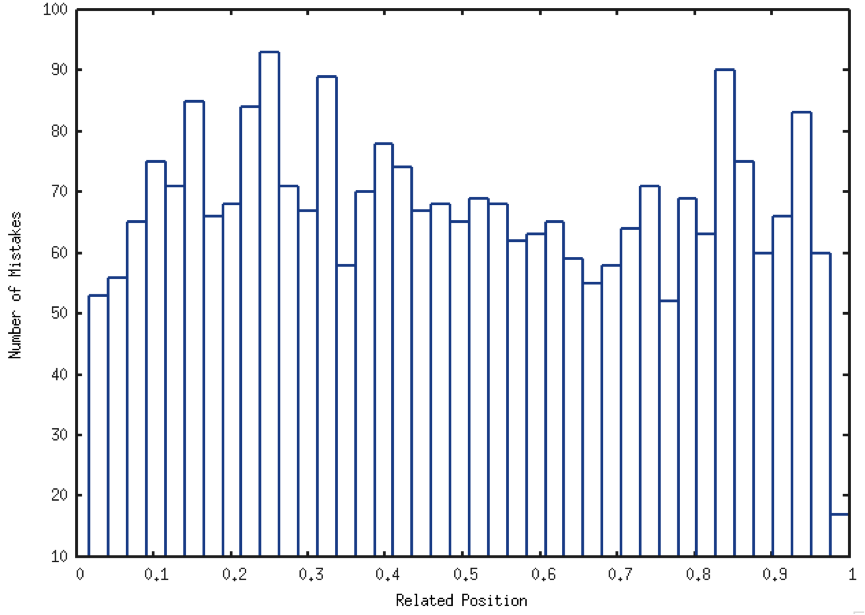
\includegraphics[scale=0.25]{indomain_pos.png} 
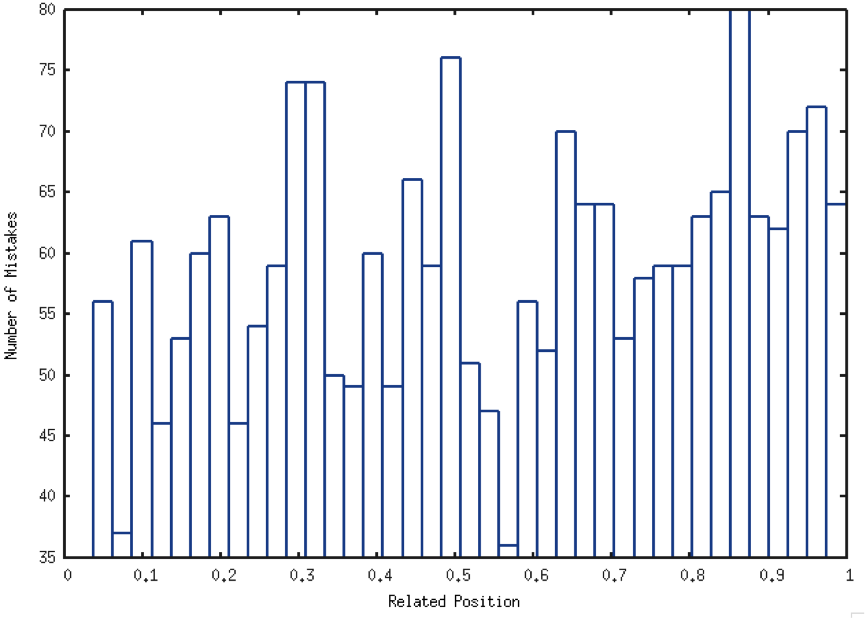
\includegraphics[scale=0.25]{outdomain_pos.png} 
\caption{Histogram of related position of wrong tags, left is in domain, right is out of domain}\label{Pos_fig}
\end{figure}

\paragraph{Not just maximum likelihood model}
In the beginning, there is a worry about whether this RNN model can pass and use the sequential information correctly. Perhaps, it just learns a maxium likelihood( most frequent ) predictor for each word or even each group of words. So we did some experiments to verify the contribution of sequential information in RNN.

\begin{itemize}
\item \textbf{Same word test}:  We choose some words with more than one  common tags and see whether our model predict those tags correctly. We tested on 'to'( possible tags are TO and IN) and 'work'(common possible tags are NN, VB and VBP). RNN predicts 'to' with 0.80 indomain accuracy and 0.77 outdomain, covering TO and IN. RNN predicts 'word' with 0.88 indomain accuracy and 0.83 outdomain, covering NN, VB and VBP.
\item \textbf{Disconnect core module test}: We disconnect the sequential information passing by ignoring the input embeddings from lower layer, and backwarded gradient from upper layer. So although it's still a RNN, there is actually no information passed between layers. We train this no-seq RNN and original RNN with 100 sentences and 100 iterations, same random seed and training parameters. The Figure \ref{Noseq_fig} shows the outdomain accuracy of two models by the number of iterations, which can be also seen from Figure \ref{Leftsize_fig}. The difference is not small. So we think the sequential information was passed and used at least partially correctly.
\end{itemize}
\begin{figure}
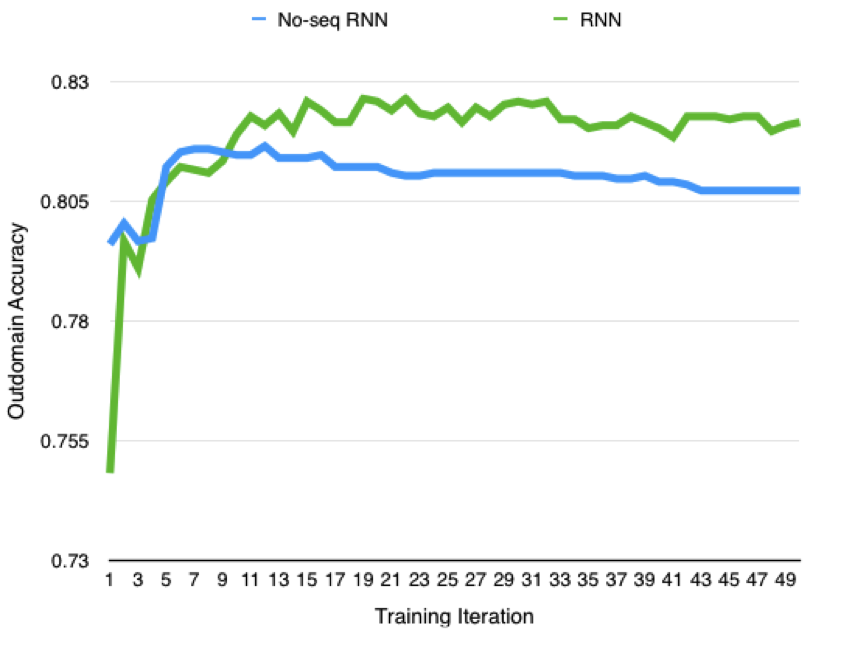
\includegraphics[scale=0.5]{outdomain_noseq.png}
\caption{Comparision of no-seq RNN and original RNN for disconnect core module test}\label{Noseq_fig}
\end{figure}

\paragraph{Different embedding size of state}
The size of state embeddings(left side of each RNN layer) is another hyper-parameter to set up. And it is important because it may determines the importance of previous sequential information comparing to the current word embedding. Figure \ref{Leftsize_fig} shows the the outdomain accuracy of two models by the number of iterations. And it looks like 20 is around the optimial size for state embeddings.
\begin{figure}
	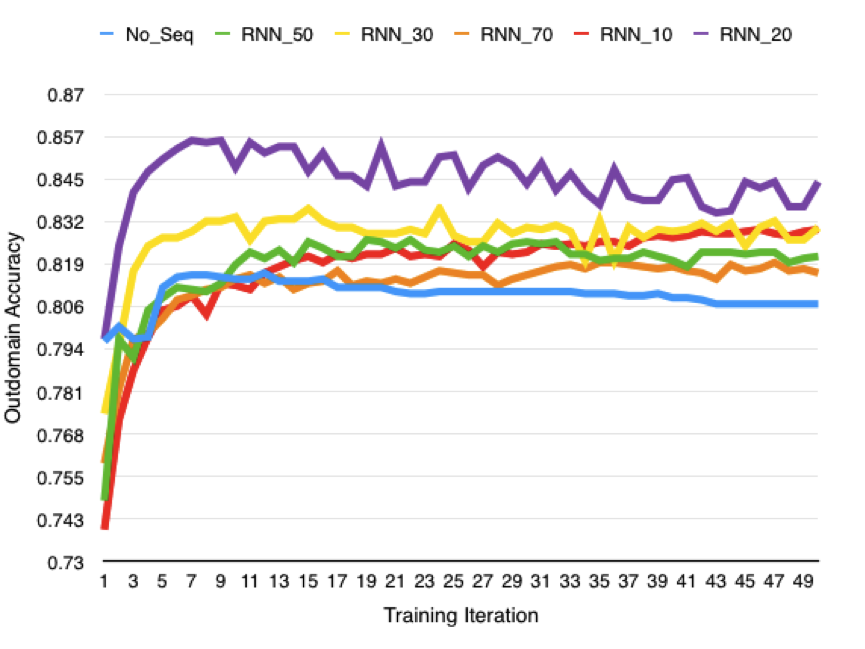
\includegraphics[scale=0.5]{outdomain_leftsize.png}
	\caption{Outdomain accuracy comparision of different state embedding size} \label{Leftsize_fig}
\end{figure}

TODO: Compare with and without updating word representations.


TODO: Specific error examples and hypotheses.





\section{Conclusion}

\section{Academic Honesty Pledge}

Honor Pledge

We pledge our honor that all the work described in this report is solely ours and
that we have given credit to all third party resources that we have used.

% include your own bib file like this:
%\bibliographystyle{acl}
%\bibliography{acl2014}

\begin{thebibliography}{}

\bibitem[\protect\citename{Aho and Ullman}1972]{Aho:72}
Alfred~V. Aho and Jeffrey~D. Ullman.
\newblock 1972.
\newblock {\em The Theory of Parsing, Translation and Compiling}, volume~1.
\newblock Prentice-{Hall}, Englewood Cliffs, NJ.

\bibitem[\protect\citename{{American Psychological Association}}1983]{APA:83}
{American Psychological Association}.
\newblock 1983.
\newblock {\em Publications Manual}.
\newblock American Psychological Association, Washington, DC.

\bibitem[\protect\citename{{Association for Computing Machinery}}1983]{ACM:83}
{Association for Computing Machinery}.
\newblock 1983.
\newblock {\em Computing Reviews}, 24(11):503--512.

\bibitem[\protect\citename{Chandra \bgroup et al.\egroup }1981]{Chandra:81}
Ashok~K. Chandra, Dexter~C. Kozen, and Larry~J. Stockmeyer.
\newblock 1981.
\newblock Alternation.
\newblock {\em Journal of the Association for Computing Machinery},
  28(1):114--133.

\bibitem[\protect\citename{Gusfield}1997]{Gusfield:97}
Dan Gusfield.
\newblock 1997.
\newblock {\em Algorithms on Strings, Trees and Sequences}.
\newblock Cambridge University Press, Cambridge, UK.

\end{thebibliography}

\end{document}
